\section{Introduction}

Large Language Models (LLMs) are indispensable in natural language processing (NLP) \citep{devlin2019bert, brown2020language, kaplan2020scaling, ouyang2022training, wei2022emergent, wei2022chain, touvron2023llama, openai2024gpt4technicalreport}, supporting applications such as chatbots \citep{anthropic2023claude, bai2023qwen, openai2024gpt4technicalreport, deepseekai2025deepseekr1incentivizingreasoningcapability}, search engines \citep{google2023bard, microsoft2023bing}, and programming assistants \citep{copilot, claude_3_7}. These models generate coherent text through \textit{inference}---the process of producing responses to user queries---which imposes significant computational demands, particularly on memory and processing resources \citep{garcia2019estimation}. Efficient inference scheduling is essential to optimize resource utilization, reduce operational costs, and minimize energy consumption \citep{strubell2019energy, desislavov2021compute}. For instance, systems like ChatGPT incur daily inference costs exceeding \$700,000 and contribute to substantial carbon emissions due to high electricity usage \citep{patel2023peeling, patterson2021carbon}. Effective scheduling strategies can address these challenges by balancing system throughput and response latency \citep{wu2022sustainable}.

Understanding the LLM inference process is essential for tackling its associated scheduling challenges. Figure~\ref{fig:intro_example} provides a step-by-step illustration of how a query is processed during inference. The process begins when a user submits a prompt—e.g., ``Is apple a fruit?''—which is then passed through several computational stages. The inference pipeline consists of two main phases:
\begin{itemize}
    \item \textbf{Prefill Phase (stage 0)}: Upon receiving the prompt, the model first tokenizes the input into a sequence of discrete units (e.g., ``Is'', ``apple'', ``a'', ``fruit'', ``?''). These tokens are then embedded and simultaneously processed in a single forward pass to compute the \textit{Key-Value (KV) cache}, which stores intermediate representations (i.e., attention keys and values) for each token. These precomputed values are critical for enabling efficient reuse during subsequent decoding steps. This phase corresponds to Stage 0 in Figure~\ref{fig:intro_example}, where all prompt tokens are embedded and their KV representations are added to the cache.

    \item \textbf{Decode Phase (stages 1 to $l^\prime$)}: After the prefill phase, the model enters the decode phase, where it generates the output one token at a time. At each stage, the model queries the existing KV cache to compute the next token, appends the new token to the output sequence, and updates the KV cache with its key-value pair. For instance, the model might first generate ``Yes'' (Stage 1), then ``it'' (Stage 2), followed by ``is'' (Stage 3), and finally the ``End of Sequence'' (EOS) token (Stage 4). This progression is depicted in the lower part of Figure~\ref{fig:intro_example}. Each token generation step involves both reading from and writing to the KV cache, resulting in a memory footprint that grows linearly with the length of the generated sequence.
\end{itemize}

Figure~\ref{fig:intro_example} also highlights key performance metrics in LLM inference:
\begin{itemize}
    \item \textbf{Time-To-First-Token (TTFT)} measures the latency from user input to the first generated token.
    \item \textbf{Latency} refers to the total time required to complete the generation of all output tokens.
    \item \textbf{Throughput} captures the average number of tokens generated per unit time.
\end{itemize}

This inference structure, particularly the growing memory requirements and sequential decoding pattern, introduces fundamental constraints on scheduling and batching. Efficient scheduling must account for both prompt heterogeneity and KV cache dynamics in order to optimize latency and resource utilization.

\begin{figure}
    \centering
    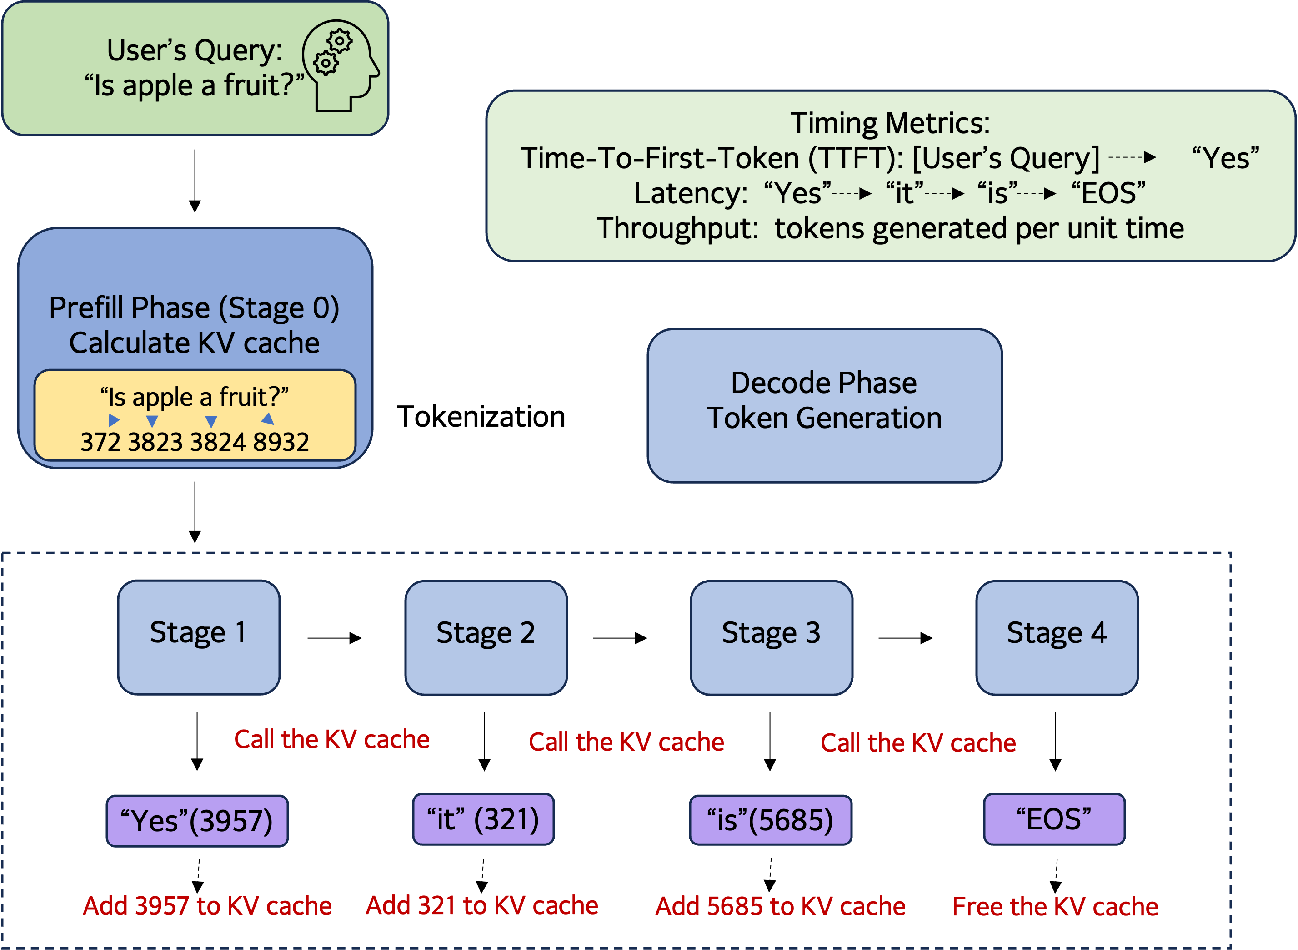
\includegraphics[width=0.6\linewidth]{Experiments_pdf/fig_intro.pdf}
    \caption{An example of LLM inference.}
    \label{fig:intro_example}
\end{figure}
The KV cache is essential for efficiency, as it prevents the model from recalculating the attention history for each new token. Without it, the computational cost would scale quadratically with the sequence length, making real-time inference infeasible. However, the expanding KV cache poses a significant scheduling challenge, as the memory footprint grows unpredictably during the decode phase. This variability, combined with stochastic prompt arrivals and differing response lengths, complicates resource allocation on hardware with finite capacity, such as GPUs. Exceeding memory limits can force the system to offload data to slower storage mediums, degrading performance and increasing latency \citep{tay2022efficient, kang2024gear, hooper2025kvquant}.

Scheduling LLM inference tasks involves grouping prompts into \textit{batches} processed concurrently on a GPU, combining prefill and decode phases to optimize resource use. This process is constrained by GPU memory limits, as the KV cache grows with each generated token, restricting the number of active prompts. Traditional scheduling methods, such as Shortest Job First (SJF), assume fixed job sizes and known processing times, making them not suitable for LLM inference where memory demands increase dynamically and output lengths are often unknown. For example, consider two prompts: one with a short input but a long, unpredictable output (e.g., ``Summarize the history of artificial intelligence''), and another with a longer input but a short output (e.g., ``Is 5 a prime number?''). In a traditional setting, SJF would prioritize the second prompt, expecting its shorter processing time to minimize average wait times. However, in LLM inference, the first prompt’s decode phase could generate hundreds of tokens, causing its KV cache to balloon over time and occupy significant memory, while the second prompt’s quick decode phase releases resources almost immediately after a longer prefill. Prioritizing the second prompt might reduce initial latency, but the first prompt’s prolonged memory usage could block other tasks, leading to GPU under-utilization and reduced throughput. Beyond SJF, other traditional methods like priority scheduling falter as they prioritize prompts without accounting for the KV cache’s unpredictable growth, potentially exhausting memory. While batching remains effective, it requires dynamic adaptation—e.g., adjusting batch sizes based on current memory usage—to accommodate the KV cache’s expansion, unlike static batching in traditional settings. These characteristics—stochastic prompt arrivals, multi-phase processing, and unpredictable resource needs—render classical operations research approaches inadequate, necessitating tailored scheduling strategies that account for dynamic memory growth and phase-specific demands.

Recent system-level optimizations for LLM inference \citep{yu2022orca, kwon2023efficient, agrawal2023sarathi, pope2023efficiently, deepseekai2024deepseekv2strongeconomicalefficient, patel2024splitwise, zhong2024distserve} focus on engineering solutions, such as batching and memory compression, but lack a rigorous mathematical foundation. 
% A notable theoretical contribution is \citet{jaillet2025onlineschedulingllminference}, which models LLM inference as an online scheduling problem with near-optimal theoretic guarantees on its average latency; however, it assumes known output lengths at arrival, limiting its applicability to real-world scenarios. 
In practice, output length predictions are imprecise or costly. For example, as shown in \cite{fu2025efficient}, the high-accuracy prediction is sensitive to the bucket size of output lengths for classification. When the output length is unknown, the performance of algorithms may degenerate significantly and performance guarantee obtained in full knowledge scenario no longer holds (see Proposition \ref{prop:unknown_lower_bound} in Section \ref{sec:nested_wait} as an example). To address this problem, we develop a fluid dynamics approximation to establish a tractable benchmark, providing insights for devising effective scheduling algorithms. Building upon this foundation, we introduce the Waiting for Accumulated Inference Threshold (WAIT) algorithm as a warm-up. This method maintains multiple thresholds to determine the scheduling order of incoming prompts, optimizing resource utilization when output lengths are known at the time of arrival. In practical applications where output lengths are not known at the time of prompt arrival, we extend our method by introducing the Nested WAIT algorithm. This algorithm constructs a hierarchical framework comprising multiple segments, each defined by distinct thresholds, to effectively manage the random prompt arrivals with unknown output lengths. It is able to ``learn" its behavior as a prompt is processed for more iterations. We show that both algorithms are asymptotically near-optimal, offering a theoretically grounded solution adaptable to practical settings. 

\subsection{Summary of Contributions}

This work contributes to LLM inference scheduling through the following contributions:
\begin{itemize}
\item \textbf{Mathematical Model}: We develop a multi-stage online scheduling model for LLM inference, accounting for queueable prompts under memory constraints (Section \ref{sec:model}). To analyze performance and inform practical algorithms, we employ a fluid dynamics approximation based on queueing theory, which serves as both an analytical tool and a performance benchmark (Section \ref{sec:fluid}).
    \item \textbf{Asymptotically Optimal Algorithms}: We develop the WAIT algorithm for known output lengths as a warm-up (Section \ref{sec:wait}) and extend it to the \textit{Nested WAIT} algorithm for unknown output lengths (Section \ref{sec:nested_wait}), both achieving asymptotic optimality under heavy traffic via novel waiting time and coupling analyses. We discuss how to extend our algorithms to more general case in Section \ref{sec:extension}.
    \item \textbf{Experimental Validation}: We evaluate our algorithms on synthetic and real-world datasets, outperforming benchmarks like vLLM \citep{kwon2023efficient} and Sarathi \citep{agrawal2023sarathi}, which are widely recognized high-performance inference engines, in average throughput using Llama2-7B on a single A100 GPU (Section \ref{sec:experiments}).
\end{itemize}
These contributions bridge operations research and machine learning, addressing analytical challenges in stochastic, memory-constrained online scheduling problems.
% The paper is structured to elucidate these advancements:
% \begin{itemize}
%     \item \textbf{Section 2} delineates the scheduling problem and its objectives.
%     \item \textbf{Section 3} details the fluid model for throughput optimization.
%     \item \textbf{Section 4} presents the booking-limit algorithm for known prompt types.
%     \item \textbf{Section 5} extends this to a nested algorithm for unknown output lengths.
%     \item \textbf{Section 6} reports numerical findings validating our approach.
%     \item \textbf{Section 7} concludes with implications and future research avenues.
% \end{itemize}

\subsection{Other Related Work}

\paragraph*{Online Scheduling Problem and Queueing System.} 
Classical online scheduling problems focus on optimally assigning jobs that arrive sequentially, each with varying completion times. In settings with stochastic arrivals, foundational studies such as \cite{devanur2009adwords,vee2010optimal,cole2014sample,balkanski2016power,lattanzi2020online} have developed algorithms that learn arrival patterns or distributions to refine scheduling strategies over time. Beyond individual job processing, works like \cite{im2013online,lucier2013efficient,liu2015online,li2020online} have explored simultaneous batching and scheduling, grouping similar jobs to enhance efficiency. Within queueing theory, fluid models serve as first-order approximations of stochastic systems, enabling near-optimal control strategies \cite{mandelbaum1998strong,maglaras2000discrete,bauerle2002optimal,liu2011network}, while heavy-traffic analysis offers insights into long-term system behavior. However, these traditional approaches fall short in addressing the unique dynamics of LLM inference, where resource requirements are dynamic due to the growing KV cache and the inference process involves distinct prefill and decode phases, unlike the static, single-phase jobs or fixed number phases and resource occupancy in classical scheduling.

\paragraph*{LLM Inference.} 
Theoretical frameworks for analyzing Large Language Model (LLM) inference are scarce, despite their widespread use, as most prior work targets system-level optimizations rather than the unique scheduling demands of LLMs. Unlike traditional scheduling, LLM inference involves stochastic arrivals, dynamic memory constraints, and multi-phase processing, complicating analytical efforts. System-level works like \cite{patel2023peeling} (``Splitwise") and \cite{zhong2024distserve} (``DistServe") split inference into prompt handling and pipeline execution, while scheduling methods such as \cite{yu2022orca}, \cite{agrawal2023sarathi}, and \cite{agrawal2024taming} use batching to boost throughput—similar to our approach. Other optimizations, e.g., \cite{deepseekai2024deepseekv2strongeconomicalefficient} with multi-head latent attention and low-rank KV compression, or \cite{fu2025efficient} with Kendall’s Tau for prioritizing prompts by predicted output lengths, focus on engineering efficiency rather than giving theoretical insight. 
% More recently, \cite{jaillet2025onlineschedulingllminference} offers a notably theoretical framework, modeling LLM inference as an online scheduling problem and analyzing an adapted shortest-job-first algorithm with near-optimal regret—yet it assumes known output lengths at arrival, a condition rarely met in practice due to their unpredictability and estimation costs (for example, another neural network may be used at the input side). 
Moreover, when full knowledge of the arriving prompts is not available, it may lead to significant performance drops (see Proposition \ref{prop:unknown_lower_bound} in Section \ref{sec:nested_wait}). Our work tries to tackle these challenges by developing a scheduling framework for the realistic case of unknown output lengths, using fluid dynamics approximations and coupling techniques from queueing theory to achieve asymptotic optimality, providing both practical relevance and a robust mathematical foundation. More recently, \cite{li2025throughput} propose a stochastic processing model for LLM inference based on a linear batch processing time approach, similar to our own. They demonstrate that work-conserving scheduling algorithms—policies designed to keep resources active whenever tasks are available—achieve optimal throughput for both individual requests and multi-agent AI workloads. Their framework extends to AI-agent scenarios such as parallel engines and fork-join models, highlighting its flexibility for complex LLM deployments. However, their analysis does not address the GPU memory usage of preempted or queued requests, particularly the memory needs of Key-Value caches for tasks awaiting processing. The study also does not explore theoretical aspects of latency metrics, such as time to first token (TTFT) or end-to-end request latency, which are important for real-time applications like interactive dialogue systems.


\subsection{Notations}
For integer $n\ge 1,$ we denote $[n]=\{1,2,\dots,n\}$ as the set of integers from $1$ to $n$. For $x\in\real$, denote $\lceil x\rceil$ as the smallest integer not smaller than $x$ and $\lfloor x\rfloor$ as the largest integer not greater than $x$. Denote $x_+=\max\{x, 0\}$. For set $S$, denote $|S|$ as its cardinality. For two functions $f(T)$ and $g(T)$, we use $f(T)=O(g(T))$ if there exists constant $c_1>0$ such that $f(T)\le c_1g(T)$ as $T\to+\infty$ and $f(T)=\Omega(g(T))$ if there exists constant $c_2>0$ such that $f(T)\ge c_2g(T)$ as $T\to +\infty$. 